\documentclass[notes,slidesec,a4]{seminar}
\usepackage[spanish]{babel}
\usepackage[utf8]{inputenc}


\usepackage{t-gsyc-6}
\usepackage{fancybox}
\usepackage{graphicx}
\graphicspath{ {./img/} }
\usepackage{graphics}
\usepackage{moreverb}
\usepackage{alltt}
\usepackage{html}
\usepackage{hthtml}
\usepackage{color}
\usepackage[usenames,dvipsnames,svgnames,table]{xcolor}
\usepackage{amsmath}
\usepackage[normalsize]{subfigure}
\usepackage{url}
\usepackage{hyperref}
\usepackage{listings}
\usepackage{multirow}

\pretolerance=100

\title{APORTES AL ENTORNO DOCENTE DE
ROBÓTICA JDEROBOT-ACADEMY}
\author{Álvaro Villamil Vuelta}

\cop{Álvaro Villamil Vuelta}
\address{a.villamil@alumnos.urjc.es}

\begin{document}
\maketitle

%%--------------------------------------------------------------

\begin{hslide}
	\slsect{Índice}
	\begin{itemize}
		\item Introducción 
		\item Objetivos
		\item Infraestructura
		\item Circuito de carreras de Fórmula 1
		\item Brazo Robótico
		\item Conclusiones
	\end{itemize}
\end{hslide}

%%--------------------------------------------------------------
\begin{hslide}
	\slsect{Introducción}
	\slsubsect{Enseñanza en Robótica}
	\begin{itemize}
		\item Secundaria: Asignatura de Tecnología; NXT, WeDo, Scratch, JdeRobot-Kids, Arduino...
		\item Grados: Algunas asignaturas; ROS y Matlab
		\item Másters: Asignaturas y cursos especializados
	\end{itemize}
\end{hslide}


\begin{hslide}
	\slsubsect{JdeRobot-Academy}
	\begin{minipage}{0.6\textwidth}
		\begin{itemize}
			\item Entorno docente de robótica universitaria orientado al aprendizaje práctico.
			\item Énfasis en la programación de la inteligencia de los robots. 
			\item Colección de prácticas variadas.
			\item Utiliza Gazebo y Python.
		\end{itemize}
	\end{minipage}
	\begin{minipage}{0.4\textwidth}
		\begin{center}
			\begin{figure}
				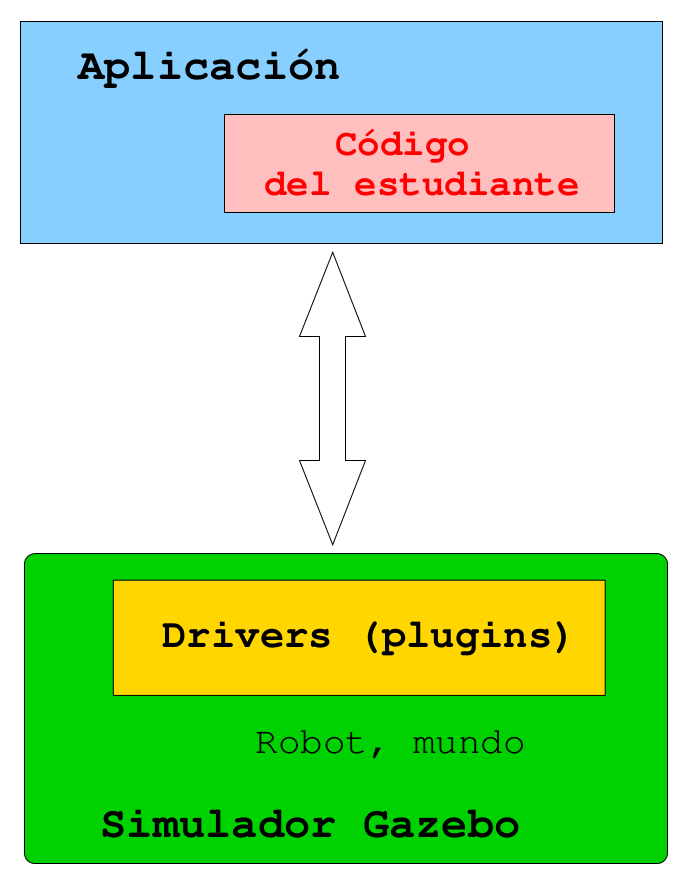
\includegraphics[width=0.8\textwidth]{esquemapracticas02.png}
			\end{figure}
		\end{center}
	\end{minipage}
\end{hslide}

\begin{hslide}
	\slsubsect{Práctica navegación local Fórmula 1.}
	\begin{itemize}
		\item Coche con sensores 
		\item Esquivar obstáculos.
		\item Algoritmo de navegación local (VFF).
	\end{itemize}
	\begin{center}
		\begin{minipage}[t]{0.55\textwidth}
			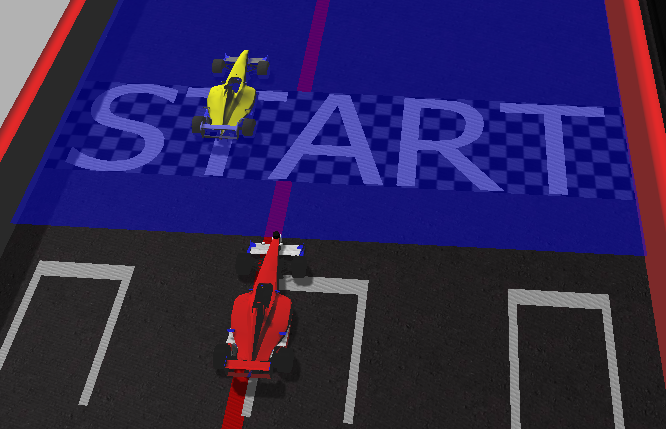
\includegraphics[width=\textwidth]{vff-gazebo.png}
		\end{minipage}
		\begin{minipage}[t]{0.25\textwidth}
			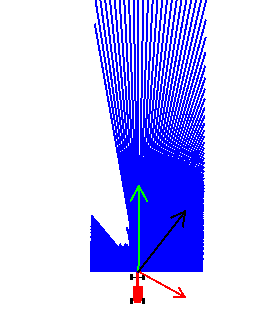
\includegraphics[width=\textwidth]{vff-gui.png}
		\end{minipage}
	\end{center}
\end{hslide}

\begin{hslide}
	\slsubsect{Práctica sigue-líneas.}
	\begin{itemize}
		\item kibuki con cámara 
		\item Seguir línea roja.
		\item Procesamiento de imágen.
	\end{itemize}
	\begin{minipage}[t]{0.47\textwidth}
		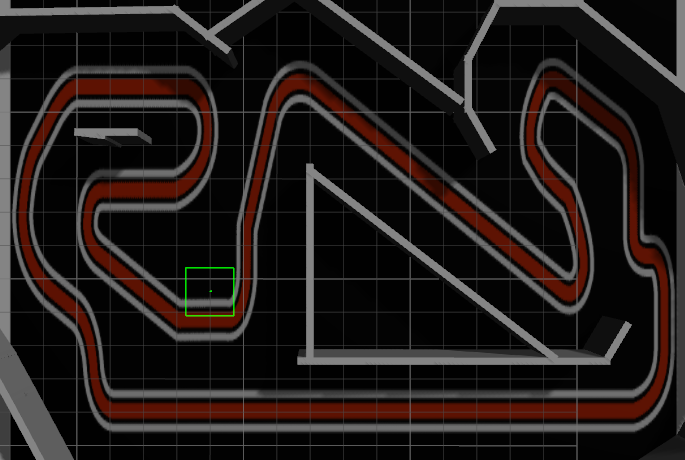
\includegraphics[width=\textwidth]{followline-world.png}
	\end{minipage}
	\begin{minipage}[t]{0.53\textwidth}
		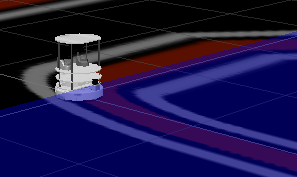
\includegraphics[width=\textwidth]{kobukiMontmelo.png}
	\end{minipage}
\end{hslide}

%%--------------------------------------------------------------
\begin{hslide}
	\slsect{Objetivo}
	Mejorar y ampliar la colección de prácticas de JdeRobot-Academy, enriqueciéndolas y aumentando el abanico de posibilidades que se ofrece al alumno.
	\begin{itemize}
		\item Mejorar la infraestructura en Gazebo de las prácticas de JdeRobot-Academy que usan coches de carreras.
		\item Diseñar y programar un teleoperador de un brazo robótico en Gazebo.
	\end{itemize}
\end{hslide}


%%--------------------------------------------------------------
\begin{hslide}
	\slsect{Infraestructura}
	\slsubsect{Blender}
	\begin{itemize}
		\item \textbf{Blender}: Programa de modelado, iluminación, renderizado, animación y creación de gráficos tridimensionales.
	\end{itemize}
	\begin{center}
		\begin{figure}
			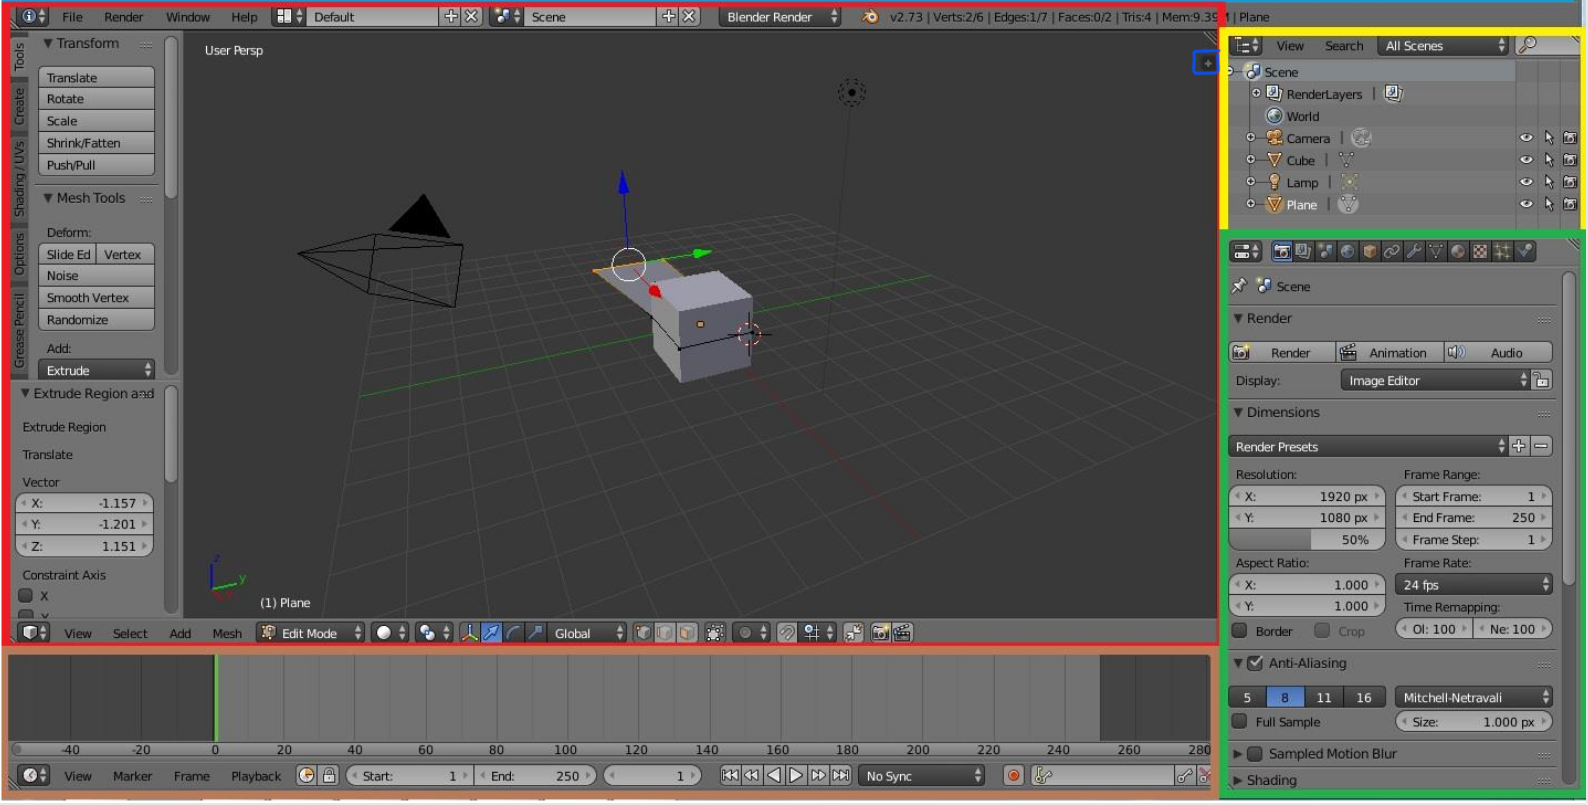
\includegraphics[width=0.6\textwidth]{InterfazBlender01.png}
		\end{figure}
	\end{center}
\end{hslide}

\begin{hslide}
	\slsubsect{Gazebo y ROS}
	\begin{itemize}
		\item \textbf{Gazebo}: Simula sensores, actuadores, robots,... en mundos virtuales.
		\item \textbf{ROS}: Es un \textit{middleware} para robots.
	\end{itemize}
	\begin{center}
		\begin{figure}
			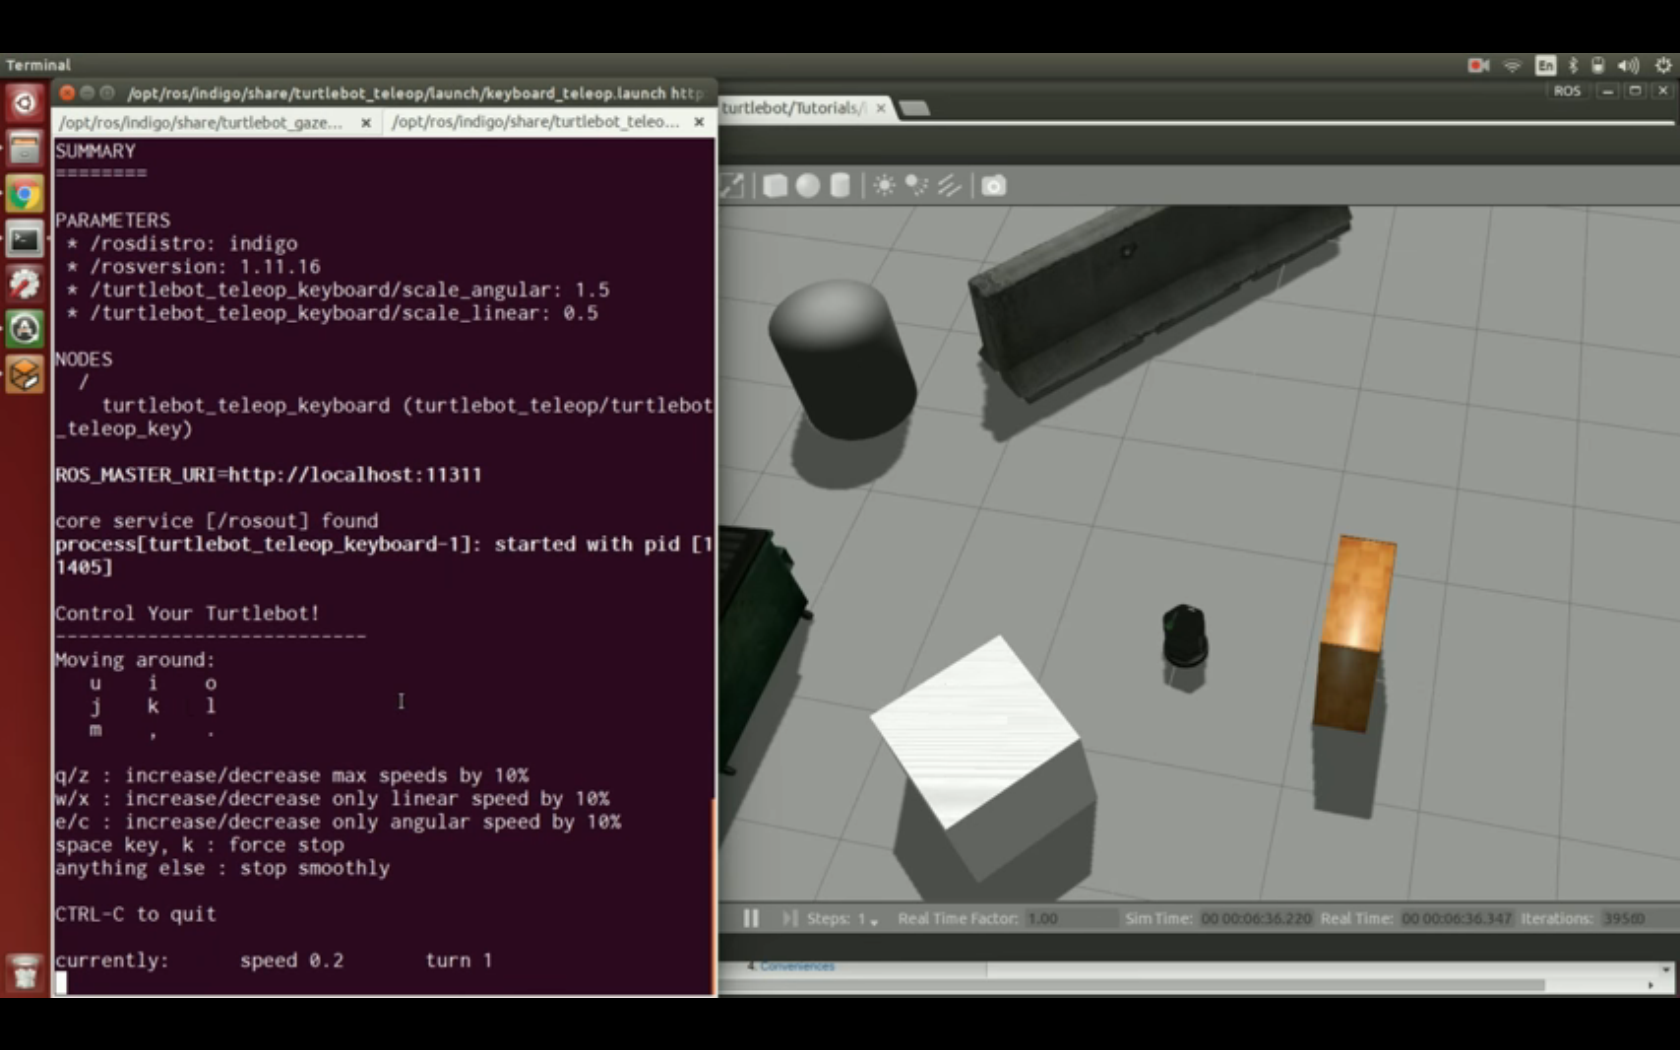
\includegraphics[width=0.6\textwidth]{ros.png}
		\end{figure}
	\end{center}
\end{hslide}

\begin{hslide}
	\slsubsect{ARIAC}
		\begin{center}(Agile Robotics for Industrial Automation Competition).	\end{center}
		Competición para probar la agilidad de los sistemas robóticos industriales.
	\begin{center}
		\begin{figure}
			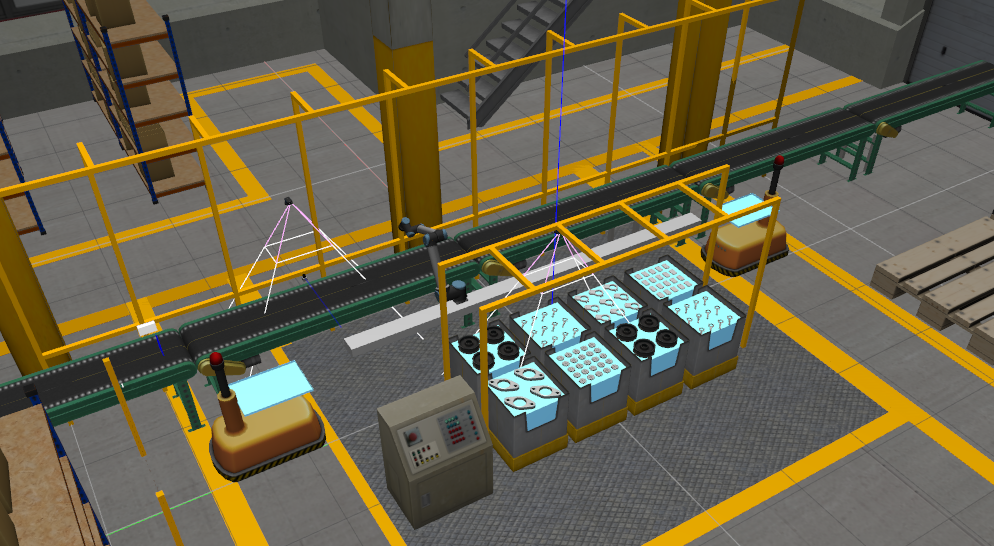
\includegraphics[width=0.6\textwidth]{ariac01.png}
		\end{figure}
	\end{center}
\end{hslide}


%%--------------------------------------------------------------
\begin{hslide}
	\slsect{Circuito de carreras de Fórmula 1}
	\begin{itemize}
		\item Reconstruir el circuito de Mónaco de forma que se pueda utilizar en:
		\begin{itemize}
			\item Práctica sigue línea.
			\item Práctica navegación local.
		\end{itemize}
		\item Creación de mundos para Gazebo que sigan el esquema de las practicas.
	\end{itemize}
\end{hslide}

\begin{hslide}
	\begin{center}
		\begin{figure}
			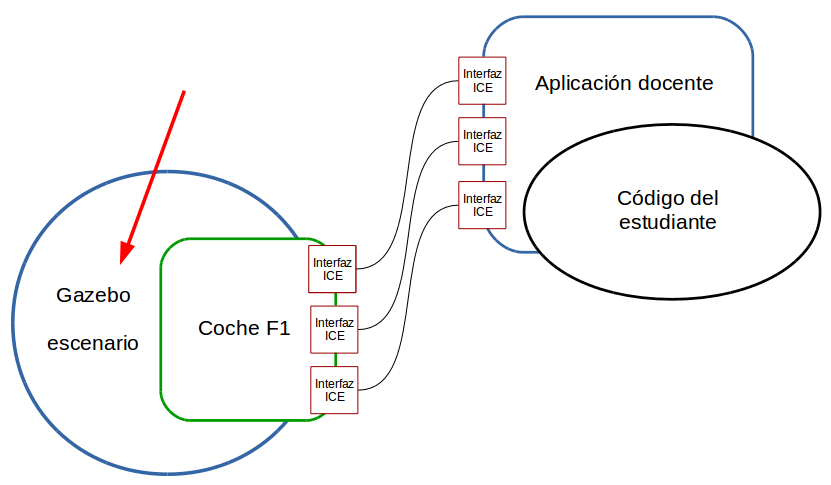
\includegraphics[width=\textwidth]{graficof1.png}
		\end{figure}
	\end{center}
\end{hslide}


\begin{hslide}
	\begin{minipage}{0.45\textwidth}
		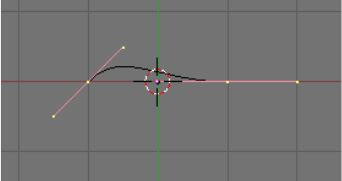
\includegraphics[width=\textwidth]{InterfazBlender05.png}
		\begin{center}
			Curva Bezier
		\end{center}
	\end{minipage}
	\begin{minipage}{0.1\textwidth}
		\begin{center}
			
\includegraphics[width=0.5\textwidth]{mas.jpg}
		\end{center}
	\end{minipage}
	\begin{minipage}{0.55\textwidth}
		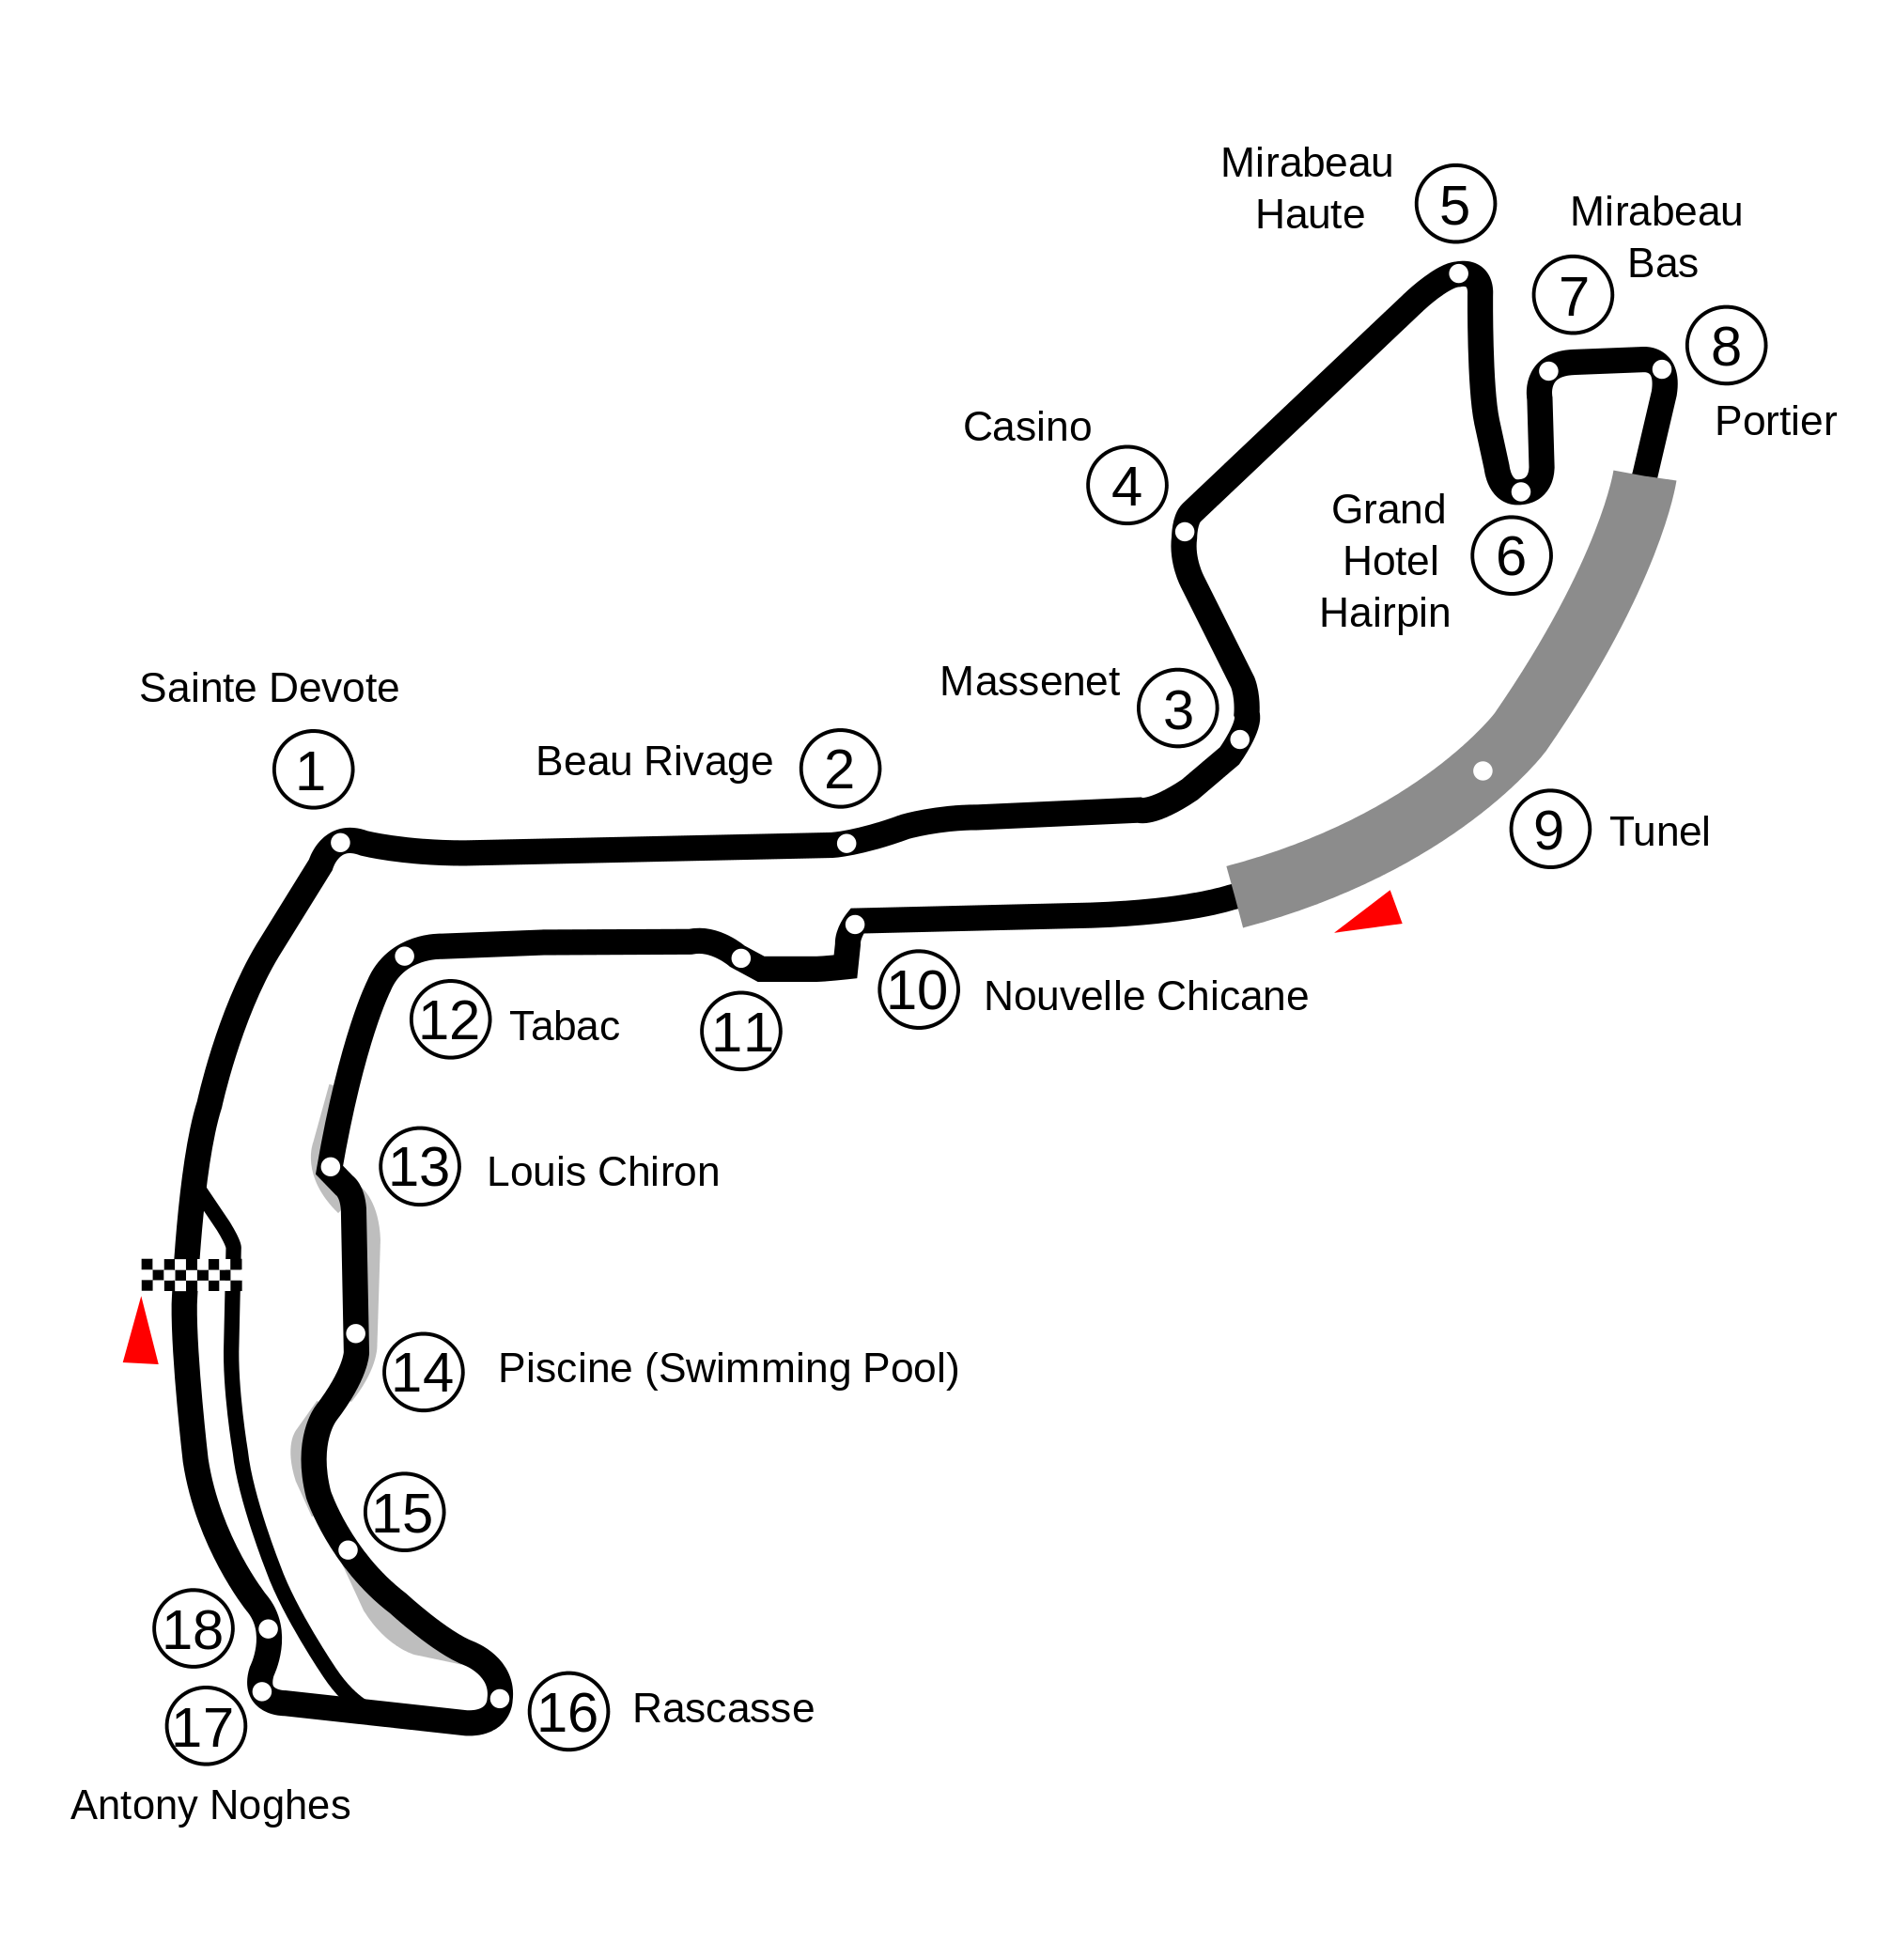
\includegraphics[width=\textwidth]{CircuitoMonaco.png}
		\begin{center}
			Plano del circuito
		\end{center}
	\end{minipage}
\end{hslide}


\begin{hslide}
	\begin{center}
		\begin{figure}
			\begin{center}
				Curva del trazado
			\end{center}
			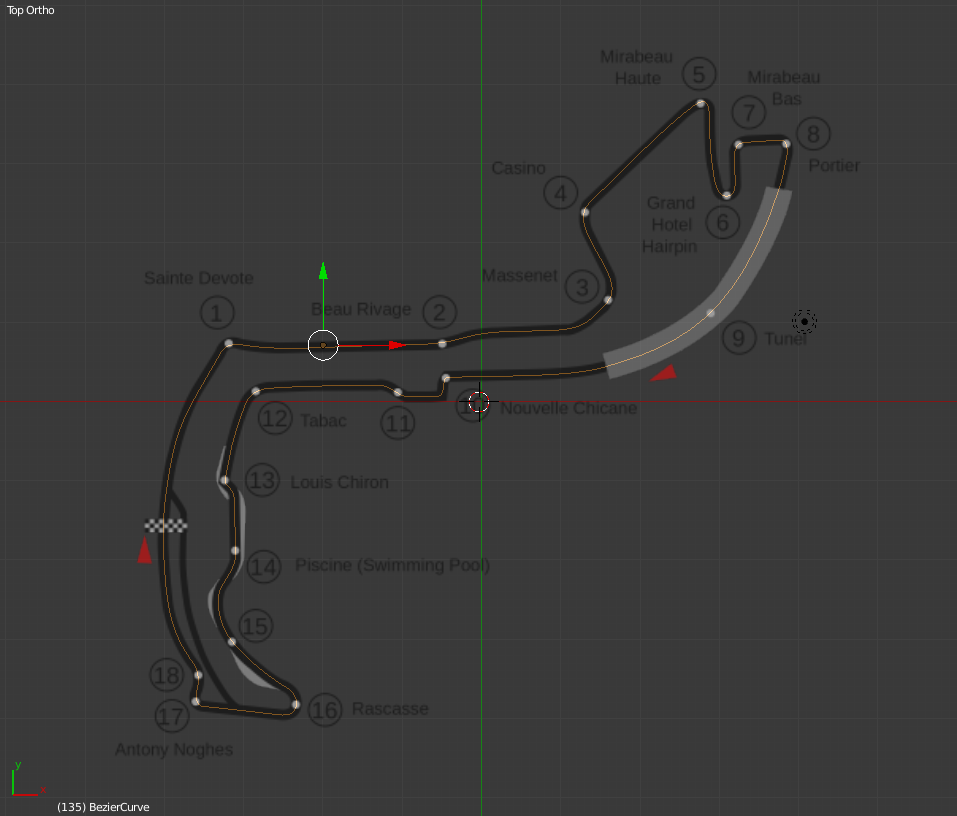
\includegraphics[width=0.75\textwidth]{MonacoTrazado.png}
		\end{figure}
	\end{center}
\end{hslide}

\begin{hslide}
**************************************************

Modelar y aplicar texturas

**************************************************
\end{hslide}

\begin{hslide}
	\begin{center}
		\begin{figure}
			\begin{center}
				Segmento del circuito
			\end{center}
			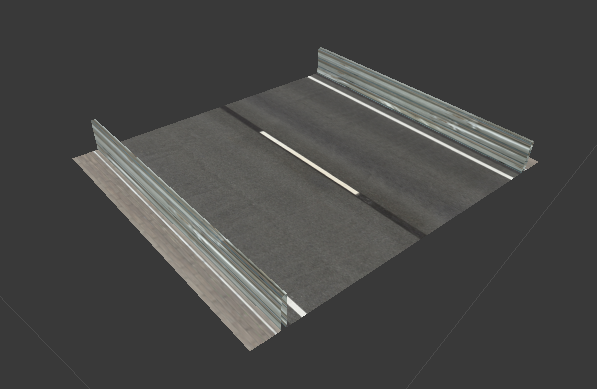
\includegraphics[width=0.82\textwidth]{MonacoSegmento.png}
		\end{figure}
	\end{center}
\end{hslide}

\begin{hslide}
	\begin{minipage}{0.5\textwidth}
		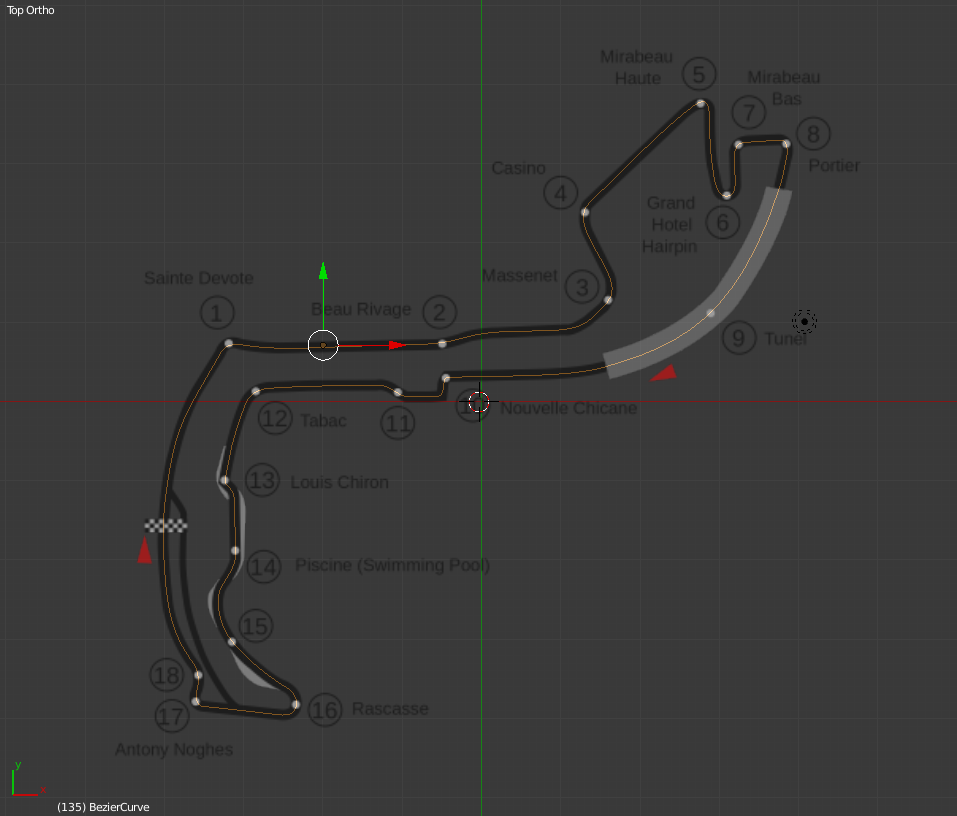
\includegraphics[width=\textwidth]{MonacoTrazado.png}
	\end{minipage}
	\begin{minipage}{0.1\textwidth}
		\begin{center}
			
\includegraphics[width=0.5\textwidth]{mas.jpg}
		\end{center}
	\end{minipage}
	\begin{minipage}{0.5\textwidth}
		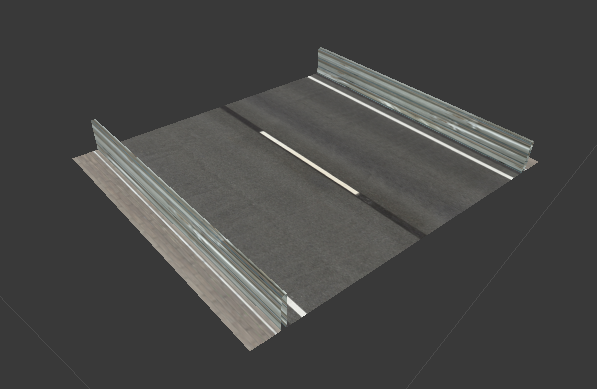
\includegraphics[width=\textwidth]{MonacoSegmento.png}
	\end{minipage}
\end{hslide}

\begin{hslide}
	\begin{center}
		\begin{figure}
			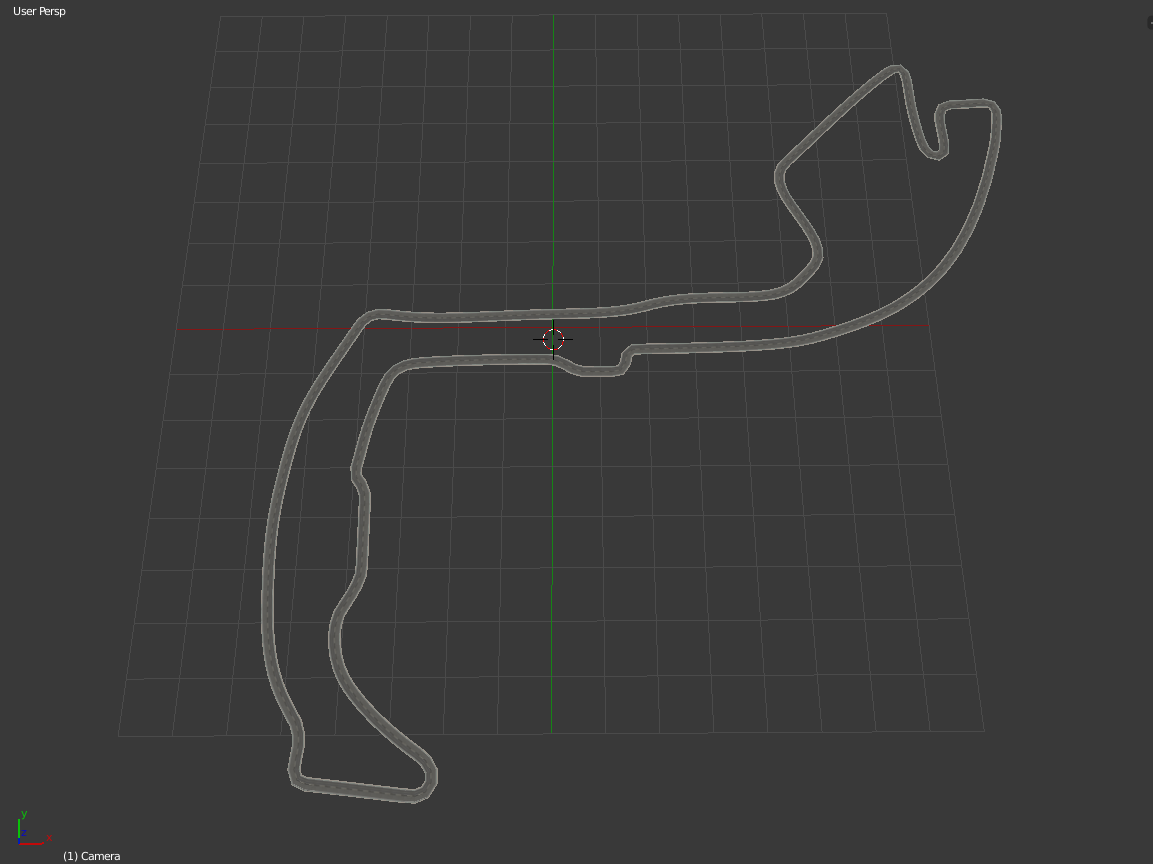
\includegraphics[width=0.82\textwidth]{Circuito00.png}
		\end{figure}
	\end{center}
\end{hslide}


\begin{hslide}
	\begin{itemize}
		\item 
	\end{itemize}
\end{hslide}

\begin{hslide}
	\slsect{Brazo robótico}
	\begin{itemize}
		\item 

		\item 
	\end{itemize}
\end{hslide}

\begin{hslide}
	\begin{center}
		\begin{figure}
			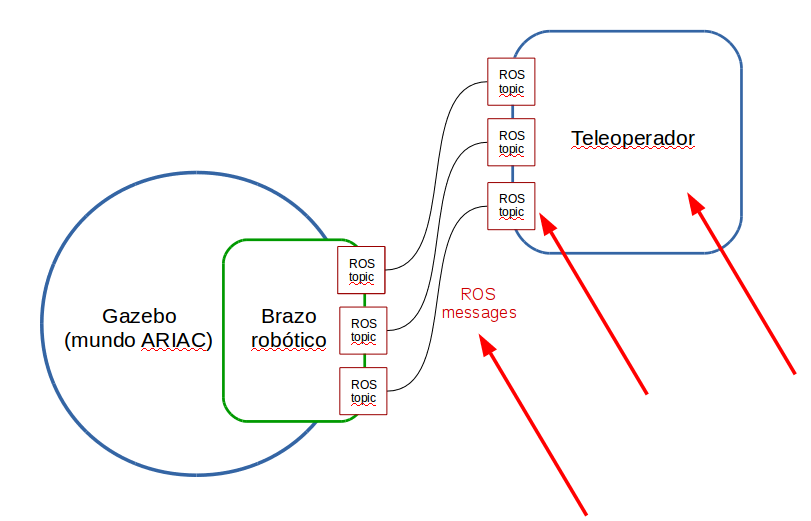
\includegraphics[width=\textwidth]{graficobrazo.png}
		\end{figure}
	\end{center}
\end{hslide}

\end{document}
